\documentclass[a4paper, 11pt]{article}
\usepackage[utf8]{inputenc} % Change according your file encoding
\usepackage{graphicx}
\usepackage{url}

%opening
\title{Distributed Systems, Advanced Course \\ 
		Project Report}
\author{KTH Royal Institute of Technology \\ 
	School of Information and Communication Technology \\
	Student:Fanti Machmount Al Samisti (fmas@kth.se) \\
	Student:Pradeep Perris (weherage@kth.se)}
\date{\today{}}

\begin{document}

\maketitle

\tableofcontents

\clearpage

\section{Introduction}

The project's goal was to realize a key value store in \textit{Kompics}. The most important properties are that it has to be distributed, replicated and comply to linearizable semantics. We were given many freedoms but we chose an easy and as little complicated as it can be implementation. \\
Our model is initially bootstrapped with a ,configurable yet, static set of nodes that comprise a group with a replication factor $\delta$. Each replication group has a segment of the key space assigned to them and a hashing function is responsible for bringing an arbitrary key value between the boundaries. \\
Finally, we support \textit{GET} and \textit{PUT} operations on the stored data. They are protected from inconsistencies(linearizable) by employing a \textit{Read-Impose Write-Consult Majority} algorithm to bring the \textit{(N,N)Atomic Register} model into our system since we can't trust our \textit{eventually perfect failure detector} so much. Essentially we have \textit{fail-noisy} semantics but it boils down to \textit{fail-silent} since we do not take into account the information from the \textit{epfd}.

\section{Design Overview}

\subsection{System Component}
The following figure depicts the overall design of the system.

{\centering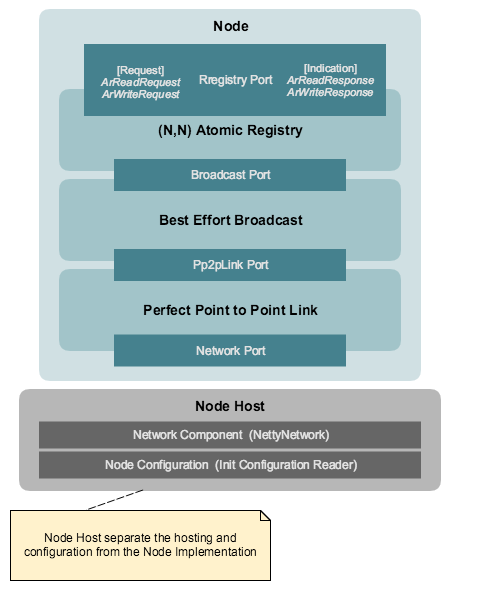
\includegraphics[scale = 0.5]{./images/design_overview.png}\par}

\subsection{Node Topology}
{\centering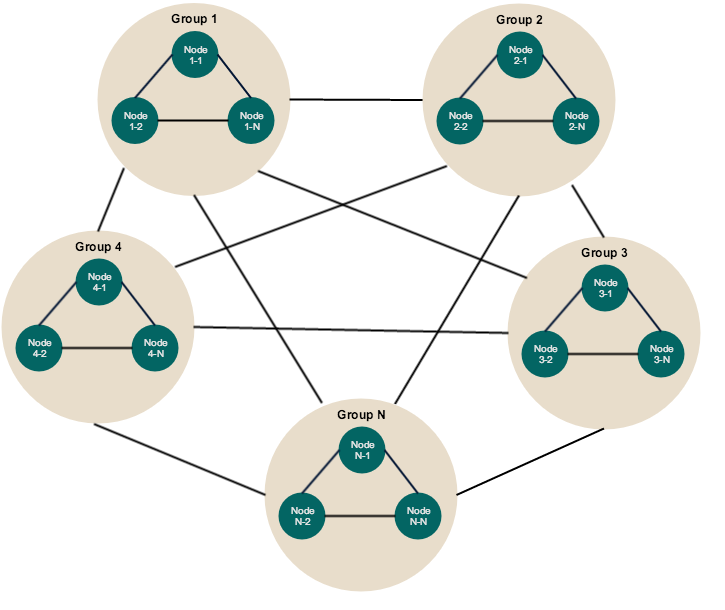
\includegraphics[scale = 0.6]{./images/node_setup.png}\par}

\section{System Abstraction and Implementation}

During our time designing and implementing the system we had a myriad of decisions to make and to motivate the `why`.

\begin{itemize}
	\item Networking protocol(TCP)
	\item Bootstrapping
	\item Group membership(Static)
	\item Failure detector($\diamond$P)
	\item Routing protocol(fully connected mesh)
	\item Replication algorithm( (N,N) Atomic Register )
\end{itemize}

Some properties have to be taken into account when deciding what algorithms to use and how to modify them according to the environment:
\begin{itemize}
	\item \textit{Network topology}: It plays a crucial role on the optimizations if its either LAN, WAN etc.
	\item \textit{Flow control}: Practical systems ask for practical solutions for example not flooding the destination with messages.
	\item \textit{Heterogenity}: Not all nodes are born equal, as they might be running on faster processors, have more memory etc.
\end{itemize}

\subsection{Perfect Point to Point Link}

All the node communication, e.g. message exchanging, is achieved by using a perfect point to point link abstraction. Since our system doesn't support any kind of reconfiguration we are working in the \textit{crash-stop} model. Additionally, we make the assumption that no messages are lost over the network as the lower levels of the operating system can handle them e.g. when being sent over \textit{TCP} by adding reliability and retransmission among others. \par 

The choice of this protocol was clear as it can support some guarantees for delivery but it doesn't come without its drawbacks. The main one is that \textit{TCP} makes assumptions about the state of the delivery buffer and combined with congestion control there might be cases of false positive crashes. Such assumptions add synchrony in an asynchronous system or in our case, partially synchronous. But as always its a matter of what algorithms the system uses and as such we have to use the appropriate abstractions. \par 

Below we see the properties that our implementation has to abide by:
\begin{itemize}
	\item \textbf{Reliable Delivery}: If a correct process p send a message m to correct process q then q eventually delivers m.(\textit{liveness})
	\item \textbf{No Duplication}: No message is delivered by a process more than once.(\textit{safety})
	\item \textbf{No Creation}: If some process q delivers a message m with sender p, then m was previously sent by process p to q.(\textit{safety})
\end{itemize}

\subsection{Best Effort Broadcast}

As pictured above our system nodes comprise one group with smaller ones to serve as replicas. The broadcasting happens only within the members of the smaller groups as sending a message to the rest of the replica groups is not useful in any shape or form. The chosen abstraction guarantees that all the correct processes will deliver as long as the sender is correct by using \textit{pp2p}. \par

Our system does not handle crashes but only detects them. This fact led us to the use of \textit{BEB} abstraction since there is no difference compared to another abstraction that can handle byzantine faults in our case. It is built on top of the \textit{pp2p} component and for each destination it issues a \textit{$\textless$pp2p|Send$\textgreater$}. \par

The properties that \textit{BEB} offers and we have to verify are:

\begin{itemize}
	\item \textbf{Validity}: If a correct process p broadcast a message m then all correct processes eventually delivers m.
	\item \textbf{No Duplication}, from \textit{pp2p}: No message is delivered more than once.
	\item \textbf{No Creation}, from \textit{pp2p}: If some process delivers a message m with sender p, then m was previously broadcast by process p to q.
\end{itemize}


\subsection{(N,N) Atomic Registry}

All the possible executions must be \textit{linearizable}. The problem we had to solve is what will happen when more than one clients send a request(\textit{GET or PUT}) to the stored data at a node level as well as at a group replication level. The only registry out of the available ones(safe, regular, atomic), the one we chose was the only one able to provide linearization semantics. \par

The replica group contains a certain number of keys(configurable in our system) but the algorithm works for one register. Due to this, we modified it to work with the hash dictionary of keys and their values by piggybacking the contextual data key to all the messages. \par

Formally, a linearizable execution guarantees:
\begin{itemize}
	\item Every read returns the last value written
	\item for any two operations x and y, if x precedes y in the execution then x also appears before y in the linearization.
\end{itemize}

The properties of \textit{NNAR} are the following:
\begin{itemize}
	\item \textit{Atomicity}: Every execution of the register is linearizable. Every failed operation appears as if it has completed or never been invoked at all. An operation appears to have completed in an instant between its invocation and completion.
	\item \textit{Termination}: If a correct process invokes an operation, then it eventually completes.
	
\end{itemize}

\subsection{Failure Detector}

Our working environment , as previously stated, is a partially synchronous system so the best way to incorporate timing assumptions is by using an \textit{eventually perfect failure detector} or $\diamond$P. At this point we found ourselves at a fork, choose a small delay to quickly react to potential failures and in time adapt to the network or choose a higher value to \textit{suspect} with a better degree of confidence but maybe detect the failure late. \par

It turns out that without implementing \textit{reconfiguration} it does not really matter if we detect a crashed node as soon as possible or well after its death. In the case we were realizing it, the importance of the delay timeout and its initial value might be crucial depending on the application constraints.

The provided properties of this abstractions are:
\begin{itemize}
	\item \textbf{Strong completeness}: Eventually, all the crashed processes will be suspected by every correct process. It is satisfied if we exclude the suspected process on timeout since it will stop responding to the \textit{heartbeats}.
	\item \textbf{Eventual strong accuracy}: Eventually, no correct node is suspected by any correct process. After the point that the system becomes synchronous, eventually all suspected correct processes will be restored and never suspected again with the increased delay timeout.
\end{itemize}

It is clear that each node cares about only its replication group and consequently $\diamond$P sends heartbeats only to the replicas. 

\subsection{Reconfiguration}

Despite not implementing any kind of crash tolerance and node addition, we decided to write down the design choices that could have gone into a theoretical system if we had, much, more time. As a reminder, the nodes are connected with a fully networked mesh(\textit{group membership service}) and comprise a number of smaller replication groups each one responsible for a different key space. \par

Starting from the base abstractions, \textit{pp2p} and \textit{beb} remain the same as they are here only to help us communicate although having the \textit{agreement} property in our broadcasting abstraction would be desirable. 

\section{System Simulations and Scenarios}
Simulation and testing of the system is carried out at each component level, starting from base of \textit{Perfect Point to Point Link} upto \textit{(N,N) Atomic Registry} components.
There are seprate Simulation Scenarious for each components,(see \textit{test/simulation} in source code bundle), that covers properties of underlying distribution abstraction.

\subsection{Perfect Point to Point Link}

As it is explained in section 3.1, the properties of \textit{Perfect Point to Point Link} to be verified are Reliability, No Duplication and No Creation.

The Reliable Delivery property is simulated in scenario \textit{pp2p/Pp2pLinkScenario.java}. It let a process instance of \textit{LinkPoint.java} to send a constant number of messages (1000) to another instance of \textit{LinkPoint.java}, and \textit{Pp2pSimulationObserver.java} listens on number of messages received at second instnce, and captures in a 
\textit{GlobalView}. GlobalView terminate and report to Simulation at successful receival of all messages.

Also this can be even proven with the standard trasport-level protocol used in the Network Layer, which is TCP. In same way No Duplication and No creation of messages are also satisfied with properties of TCP.

\subsection{Best Effort Broadcast}

The properties of \textit{Best Effort Broadcast} to be verfied are Validity, No Duplication and No Creation.

The Validy property of the component is simulated and verified in \textit{BebScenario.java}. Within \textit{beb/BebScenario.java}, it creates a constant number of (1000) of \textit{beb/BebPointHost.java} instances as the receivers and let another instance of \textit{beb/BebPointHost.java} to broadcast a message. \textit{BebSimulationObserver.java} simply verifies that all receviers are received with the broadcast message. No Duplication and No Creation properties are derived from the underlyine \textit{Perfect Point to Point Link} component.

\textit{Best Effort Broadcast} ensures only delivery of messages amoung correct processes. The simulation [TODO] verifiy this.

\subsection{(N,N) Atomic Registry}

As it is explained in section 3.3, the properties of \textit{(N,N) Atomic Registry (NNAR)} are Atomicity and Termination. \textit{NNAR} is a strict generalization of \textit{(1,N) Atomic Registry (ONAR)}, as the every execution of \textit{ONAR} is also an execution of \textit{NNAR}. Therefore, \textit{Ordering} property of \textit{ONAR} should be verified in \textit{NNAR} with a single writer.

The simulation scenario in \textit{register/SimpleReadWriteScenario.java} simply verify the termincation of Read/Write operation. Also the simulation \textit{register/WriteAfterReadAllScenario.java} further verify after a write operation, eventually all Reader processors received the written value each registry node.

The scenario \textit{register/TwoWritesLastReadScenario.java} covers the following execution.

{\centering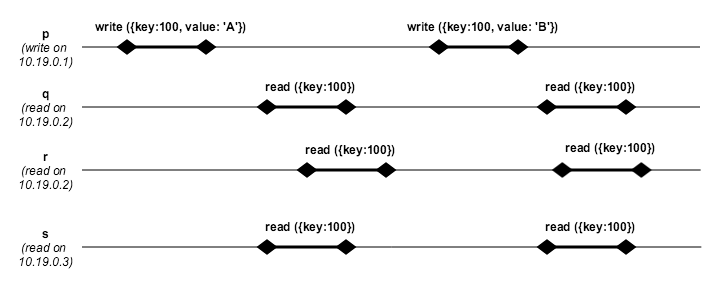
\includegraphics[scale = 0.5]{./images/2writers_read_last.png}\par}

\textit{register/TwoWritesLastReadObserver.java} verifies that last read always return the last written value. That is, it prevents old value being read, which covers \textit{Ordering} property of \textit{ONAR}.

The scenario (TODO) covers the following execution. The lineriazability is captured in (TODO) Observer and verify the execution.

{\centering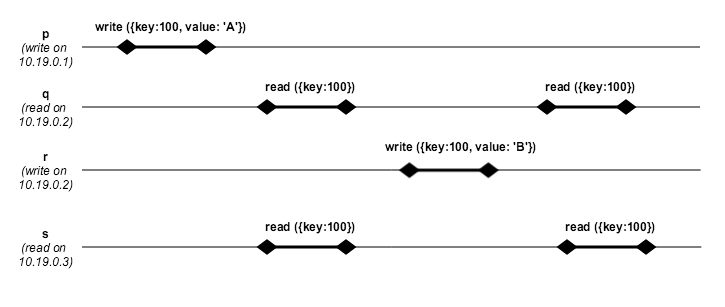
\includegraphics[scale = 0.5]{./images/mwriters_read.png}\par}


(TODO, concurrent write/read, should return last write, but follows the last read value)

{\centering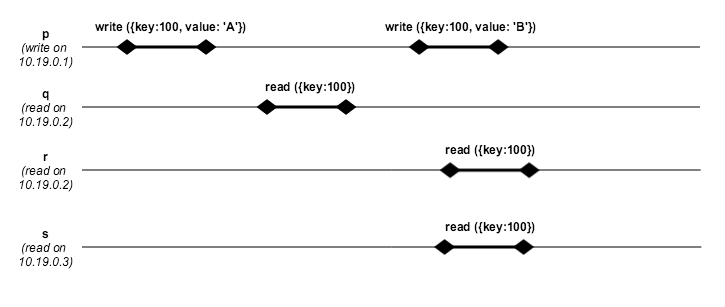
\includegraphics[scale = 0.5]{./images/concurent_read_write.png}\par}

{\centering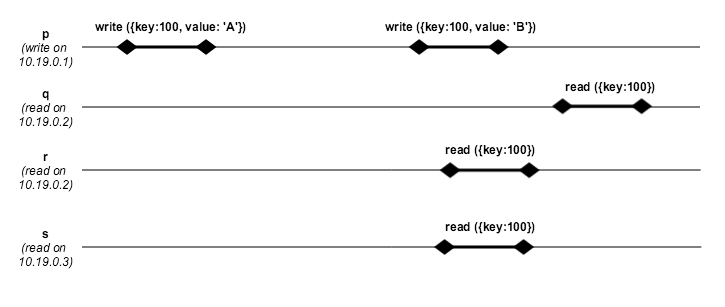
\includegraphics[scale = 0.5]{./images/concurent_read_write2.png}\par}


(TODO, Failed writers appear as never invoked or completed)
{\centering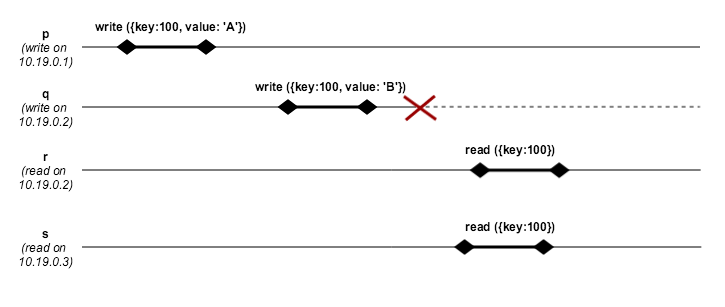
\includegraphics[scale = 0.5]{./images/failed_writer.png}\par}

Our NNAR is improved to work with value of hash dictionary. Therefore, it should allow Read/Write on multiple key values simultenously, it should not block the Read or Write operation with low rid.

{\centering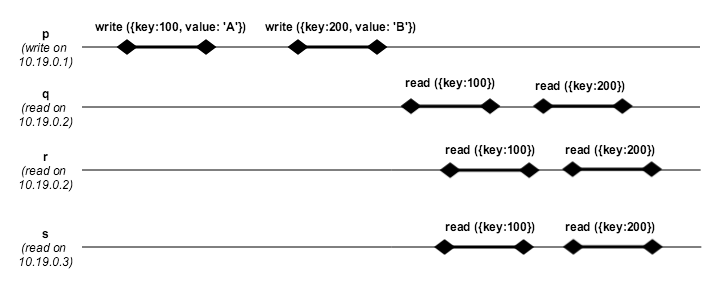
\includegraphics[scale = 0.5]{./images/mkey_writes.png}\par}


\section{Conclusions}

The open ended nature of the project was a blessing and a curse. The freedom we had helped us develop critical thinking on distributed systems as well as reasoning and insight on why something works(usually does not). On the contrary, due to  this being our first real world project with an actual implementation, initially it felt like being dropped in the desert with the task to build a place to live. \par

After finding our bearings with \textit{Kompics} and figuring out its quirks development went smooth with the only headache being how to test and debug the system. Last thing before moving to the meat of the summary is how straightforward it was to implement an algorithm from the book on 1 to 1 translation. \par

Developing a fully realized system, despite of it having a steep(for us) learning curve, taught us a myriad of things. 

\end{document}
